% ============================================================
% CHƯƠNG 4: XÂY DỰNG, TRIỂN KHAI VÀ KIỂM THỬ HỆ THỐNG
% ============================================================

\chapter{Xây dựng, triển khai và kiểm thử hệ thống}

\section{Cài đặt hệ thống}

\subsection{Khái quát tổng thể}

Hệ thống SmartNutri được cài đặt dưới dạng ba thành phần riêng biệt:

\begin{enumerate}
    \item \textbf{Ứng dụng di động (Flutter):} Được build thành file APK (Android) hoặc IPA (iOS), cài đặt trực tiếp trên thiết bị người dùng.
    \item \textbf{Backend (Firebase):} Được triển khai trên nền tảng đám mây của Google Firebase, bao gồm Firestore, Authentication, Storage, và Cloud Functions.
    \item \textbf{Trang quản trị (React):} Được build thành static files và deploy lên Firebase Hosting.
\end{enumerate}

\subsection{Kiến trúc hệ thống}

Ứng dụng Flutter tuân theo kiến trúc \textbf{feature-first} với các tầng rõ ràng:

\begin{itemize}
    \item \textbf{Tầng Presentation:} Chứa các widget Flutter cho từng màn hình (pages) và các component dùng chung (widgets).
    \item \textbf{Tầng Business Logic:} Sử dụng ChangeNotifier/StateNotifier để quản lý state, xử lý logic nghiệp vụ.
    \item \textbf{Tầng Service:} Chứa các service class để tương tác với Firebase (AuthService, FirestoreService, StorageService) và các API bên ngoài (GeminiService).
    \item \textbf{Tầng Model:} Định nghĩa các data class tương ứng với document Firestore.
\end{itemize}

\begin{figure}[H]
    \centering
    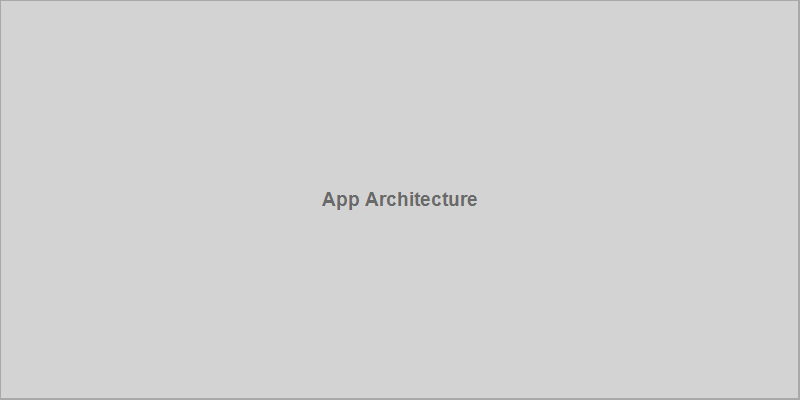
\includegraphics[width=0.85\textwidth]{assets/diagrams/app_architecture.png}
    \caption{Kiến trúc phân tầng ứng dụng Flutter}
    \label{fig:app_architecture}
\end{figure}

\subsection{Các thuộc tính chất lượng được hỗ trợ}

\begin{itemize}
    \item \textbf{Tính khả dụng (Usability):} Giao diện tiếng Việt, thiết kế trực quan, luồng người dùng đơn giản. Onboarding flow giúp cá nhân hóa trải nghiệm.
    \item \textbf{Tính hiệu năng (Performance):} Sử dụng Firestore caching cho phép truy cập dữ liệu offline. Lazy loading hình ảnh từ Firebase Storage.
    \item \textbf{Tính bảo mật (Security):} Firebase Authentication + Firestore Security Rules đảm bảo mỗi người dùng chỉ truy cập được dữ liệu của chính mình. API key nhạy cảm được giấu phía Cloud Functions.
    \item \textbf{Tính khả chuyển (Portability):} Flutter hỗ trợ cả Android và iOS từ một codebase. Admin web chạy trên mọi trình duyệt hiện đại.
    \item \textbf{Tính khả bảo trì (Maintainability):} Code được tổ chức theo feature module, dễ dàng mở rộng và bảo trì. TypeScript cho Cloud Functions và Admin Web giúp phát hiện lỗi sớm.
\end{itemize}

\subsection{Triển khai hệ thống}

\subsubsection{Triển khai Firebase}

\begin{enumerate}
    \item Cấu hình Firebase project trên Firebase Console.
    \item Thiết lập Authentication providers (Email/Password, Google Sign-In).
    \item Deploy Firestore Security Rules và Indexes.
    \item Deploy Storage Rules.
    \item Deploy Cloud Functions lên Firebase.
    \item Deploy Admin Web lên Firebase Hosting.
\end{enumerate}

\subsubsection{Build ứng dụng di động}

\begin{enumerate}
    \item Cấu hình `google-services.json` (Android) trong project Flutter.
    \item Chạy `flutter build apk --release` để tạo APK production.
    \item Phân phối qua Google Play Store hoặc cài đặt trực tiếp.
\end{enumerate}

\section{Kiểm thử hệ thống và trình bày kết quả thực nghiệm}

\subsection{Kiểm thử chức năng}

\subsubsection{Kiểm thử xác thực và phân quyền}

\begin{longtable}{|p{2cm}|p{3cm}|p{2.5cm}|p{3cm}|p{2.5cm}|p{1.5cm}|}
    \hline
    \textbf{Mã TC} & \textbf{Chức năng} & \textbf{Dữ liệu vào} & \textbf{Kết quả mong đợi} & \textbf{Kết quả thực tế} & \textbf{Trạng thái} \\
    \hline
    \endhead
    \hline
    \endfoot
    AUTH-01 & Đăng ký với email hợp lệ & Email: test@example.com, Password: Test123 & Tạo tài khoản thành công, chuyển đến Onboarding & Chưa có bằng chứng kiểm thử thực tế & Chưa xác nhận \\
    \hline
    AUTH-02 & Đăng ký với email đã tồn tại & Email: existing@example.com & Hiển thị lỗi ``Email đã được sử dụng'' & Chưa có bằng chứng kiểm thử thực tế & Chưa xác nhận \\
    \hline
    AUTH-03 & Đăng ký với mật khẩu yếu & Password: 123 & Hiển thị lỗi ``Mật khẩu phải có ít nhất 6 ký tự'' & Chưa có bằng chứng kiểm thử thực tế & Chưa xác nhận \\
    \hline
    AUTH-04 & Đăng nhập đúng thông tin & Email + Password hợp lệ & Đăng nhập thành công, vào màn hình chính & Chưa có bằng chứng kiểm thử thực tế & Chưa xác nhận \\
    \hline
    AUTH-05 & Đăng nhập sai mật khẩu & Password sai & Hiển thị lỗi ``Sai thông tin đăng nhập'' & Chưa có bằng chứng kiểm thử thực tế & Chưa xác nhận \\
    \hline
    AUTH-06 & Đăng nhập bằng Google & Tài khoản Google hợp lệ & Đăng nhập thành công & Chưa có bằng chứng kiểm thử thực tế & Chưa xác nhận \\
    \hline
    AUTH-07 & Đăng xuất & -- & Về màn hình đăng nhập & Chưa có bằng chứng kiểm thử thực tế & Chưa xác nhận \\
    \hline
\end{longtable}

\subsubsection{Kiểm thử luồng nghiệp vụ chính}

\begin{longtable}{|p{2cm}|p{3cm}|p{2.5cm}|p{3cm}|p{2.5cm}|p{1.5cm}|}
    \hline
    \textbf{Mã TC} & \textbf{Chức năng} & \textbf{Dữ liệu vào} & \textbf{Kết quả mong đợi} & \textbf{Kết quả thực tế} & \textbf{Trạng thái} \\
    \hline
    \endhead
    \hline
    \endfoot
    BIZ-01 & Hoàn thành Onboarding & Thông tin cá nhân & Dữ liệu được lưu, mục tiêu được thiết lập & Chưa có bằng chứng kiểm thử thực tế & Chưa xác nhận \\
    \hline
    BIZ-02 & Quét món ăn & Ảnh món ăn & AI nhận diện và trả về thông tin dinh dưỡng & Chưa có bằng chứng kiểm thử thực tế & Chưa xác nhận \\
    \hline
    BIZ-03 & Thêm món ăn thủ công & Tên món + khẩu phần & Món ăn được thêm vào nhật ký & Chưa có bằng chứng kiểm thử thực tế & Chưa xác nhận \\
    \hline
    BIZ-04 & Xem nhật ký ngày & -- & Hiển thị danh sách món đã ăn trong ngày & Chưa có bằng chứng kiểm thử thực tế & Chưa xác nhận \\
    \hline
    BIZ-05 & Xem thống kê dinh dưỡng & -- & Hiển thị biểu đồ calo, macro & Chưa có bằng chứng kiểm thử thực tế & Chưa xác nhận \\
    \hline
    BIZ-06 & Thêm món yêu thích & Chọn món từ danh sách & Món được thêm vào danh sách yêu thích & Chưa có bằng chứng kiểm thử thực tế & Chưa xác nhận \\
    \hline
    BIZ-07 & Chat với AI dinh dưỡng & Câu hỏi về dinh dưỡng & AI trả lời câu hỏi phù hợp & Chưa có bằng chứng kiểm thử thực tế & Chưa xác nhận \\
    \hline
\end{longtable}

\subsubsection{Kiểm thử chức năng Admin}

\begin{longtable}{|p{2cm}|p{3cm}|p{2.5cm}|p{3cm}|p{2.5cm}|p{1.5cm}|}
    \hline
    \textbf{Mã TC} & \textbf{Chức năng} & \textbf{Dữ liệu vào} & \textbf{Kết quả mong đợi} & \textbf{Kết quả thực tế} & \textbf{Trạng thái} \\
    \hline
    \endhead
    \hline
    \endfoot
    ADM-01 & Thêm thực phẩm mới & Thông tin món ăn đầy đủ & Thực phẩm được thêm vào CSDL & Chưa có bằng chứng kiểm thử thực tế & Chưa xác nhận \\
    \hline
    ADM-02 & Sửa thông tin thực phẩm & Thông tin cập nhật & Thực phẩm được cập nhật & Chưa có bằng chứng kiểm thử thực tế & Chưa xác nhận \\
    \hline
    ADM-03 & Xóa thực phẩm & ID thực phẩm & Thực phẩm bị đánh dấu inactive & Chưa có bằng chứng kiểm thử thực tế & Chưa xác nhận \\
    \hline
    ADM-04 & Xem danh sách người dùng & -- & Hiển thị danh sách người dùng đã đăng ký & Chưa có bằng chứng kiểm thử thực tế & Chưa xác nhận \\
    \hline
\end{longtable}

\subsection{Kiểm thử hiệu năng}

Phần kiểm thử hiệu năng chưa được thực hiện bằng công cụ đo chuyên dụng. Do đó, báo cáo chưa đưa ra số liệu định lượng về thời gian khởi động ứng dụng, thời gian phản hồi API hoặc mức tiêu thụ bộ nhớ.

\subsection{Kiểm thử bảo mật}

Phần kiểm thử bảo mật chưa có biên bản kiểm thử độc lập. Các nội dung cần được xác minh trong giai đoạn tiếp theo bao gồm: quyền truy cập dữ liệu theo Firestore Security Rules, xác thực người dùng, và khả năng bảo vệ các khóa API nhạy cảm.

\subsection{Kiểm thử tích hợp}

Kiểm thử tích hợp end-to-end giữa ứng dụng di động, Firebase và dịch vụ AI chưa được ghi nhận bằng biên bản chính thức. Báo cáo hiện chỉ mô tả kế hoạch kiểm thử, chưa kết luận trạng thái đạt hay không đạt cho nhóm kiểm thử này.

\subsection{Kiểm thử giao diện}

Kiểm thử giao diện trên nhiều kích thước màn hình và thiết bị khác nhau chưa được ghi nhận đầy đủ. Phần này cần được bổ sung sau khi có kết quả kiểm thử thực tế trên thiết bị hoặc trình giả lập.

\section{Giao diện hệ thống}

\subsection{Màn hình đăng nhập và đăng ký}

\begin{figure}[H]
    \centering
    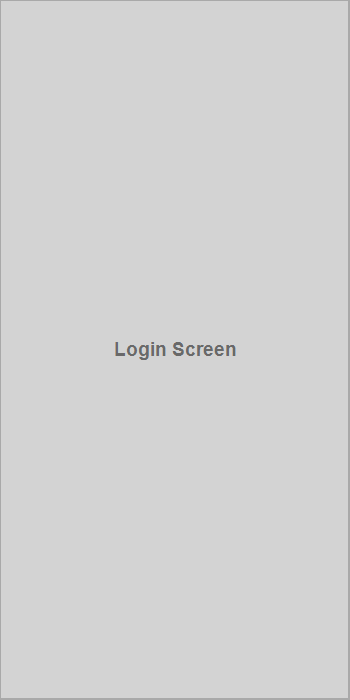
\includegraphics[width=0.35\textwidth]{assets/screenshots/login_screen.png}
    \caption{Màn hình đăng nhập}
    \label{fig:login_screen}
\end{figure}

[TODO: Bổ sung screenshot và mô tả cho các màn hình: Onboarding, Trang chủ, Quét món ăn, Nhật ký, Thống kê, Chatbot AI, Trang Admin.]

\begin{figure}[H]
    \centering
    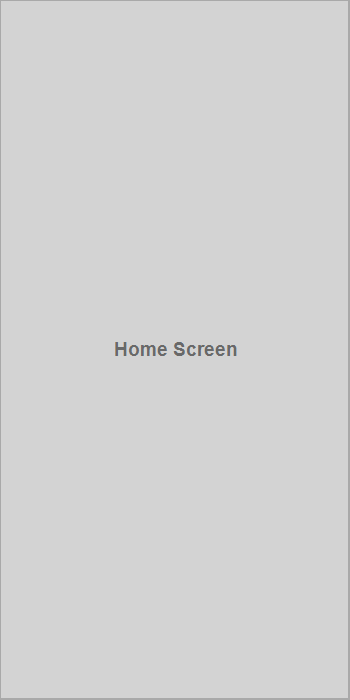
\includegraphics[width=0.35\textwidth]{assets/screenshots/home_screen.png}
    \caption{Màn hình trang chủ}
    \label{fig:home_screen}
\end{figure}

\begin{figure}[H]
    \centering
    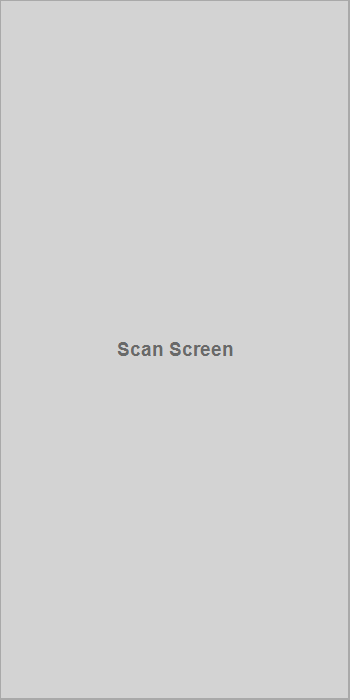
\includegraphics[width=0.35\textwidth]{assets/screenshots/scan_screen.png}
    \caption{Màn hình quét món ăn}
    \label{fig:scan_screen}
\end{figure}

\begin{figure}[H]
    \centering
    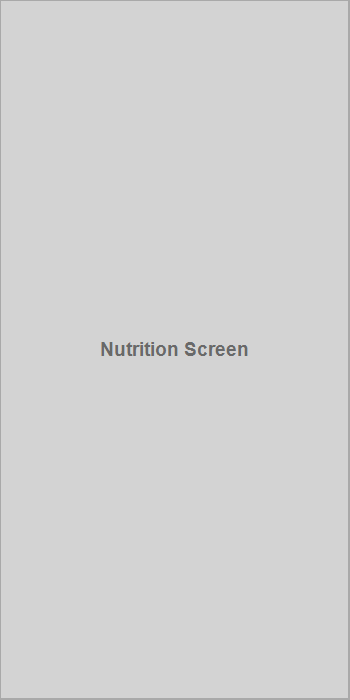
\includegraphics[width=0.35\textwidth]{assets/screenshots/nutrition_screen.png}
    \caption{Màn hình theo dõi dinh dưỡng}
    \label{fig:nutrition_screen}
\end{figure}
